\documentclass{article}
\usepackage{graphicx}
\usepackage{amsmath}
\usepackage{lscape}
\usepackage{hyperref}

\title{Análisis Económico y Estrategia de Trading Basada en la Situación Actual del Petróleo}
\author{Analista Financiero}
\date{\today}

\begin{document}

\maketitle

\tableofcontents

\section{Resumen Económico}
El contexto económico global está marcado por una situación geopolítica delicada, como la tensión entre Irán e Israel, que típicamente genera incertidumbre en los mercados energéticos. Sin embargo, como se menciona en el video, la prima de guerra en el petróleo sigue siendo baja debido a varios factores:
\begin{itemize}
    \item Estados Unidos se ha convertido en el mayor productor de petróleo, lo que ha reducido la dependencia global de regiones volátiles.
    \item Los gobiernos occidentales han optado por liberar reservas estratégicas de petróleo para estabilizar los precios en caso de un aumento repentino.
    \item Las sanciones a países productores como Venezuela han sido relajadas para incrementar la oferta global.
    \item Los mercados de derivados de petróleo han crecido significativamente, multiplicando por 15 los volúmenes negociados desde 2006, lo que ha permitido a los consumidores cubrirse ante fluctuaciones.
\end{itemize}
Además, la mejora en los sistemas de información vía satélite ha reducido la incertidumbre sobre los flujos de petróleo, contribuyendo a una menor volatilidad en los precios.

\section{Análisis de Mercado}
\subsection{Mercado del Petróleo}
A pesar del riesgo geopolítico en Medio Oriente, el precio del petróleo ha mostrado un comportamiento lateral bajista, manteniéndose más cerca de los \$60 por barril que de los \$100. Este comportamiento se debe en gran medida a los factores mencionados previamente, que han contribuido a mantener una prima de guerra baja.

\subsection{Mercados Financieros Globales}
El mercado de acciones ha reaccionado con cierta calma a la situación del petróleo, ya que la oferta no se ha visto significativamente afectada. Sin embargo, sectores como el energético y el de transporte han mostrado cierta volatilidad debido a las fluctuaciones en los precios del crudo.

Las divisas de países exportadores de petróleo como Rusia y Canadá han mostrado correlación con las fluctuaciones del precio del crudo, presentando oportunidades para operaciones de arbitraje en pares de divisas relacionadas.

\subsection{Gráficos y Tablas}
A continuación se presentan gráficos de la evolución reciente del precio del petróleo, junto con la correlación de las divisas de países exportadores:

\begin{figure}[h!]
\centering
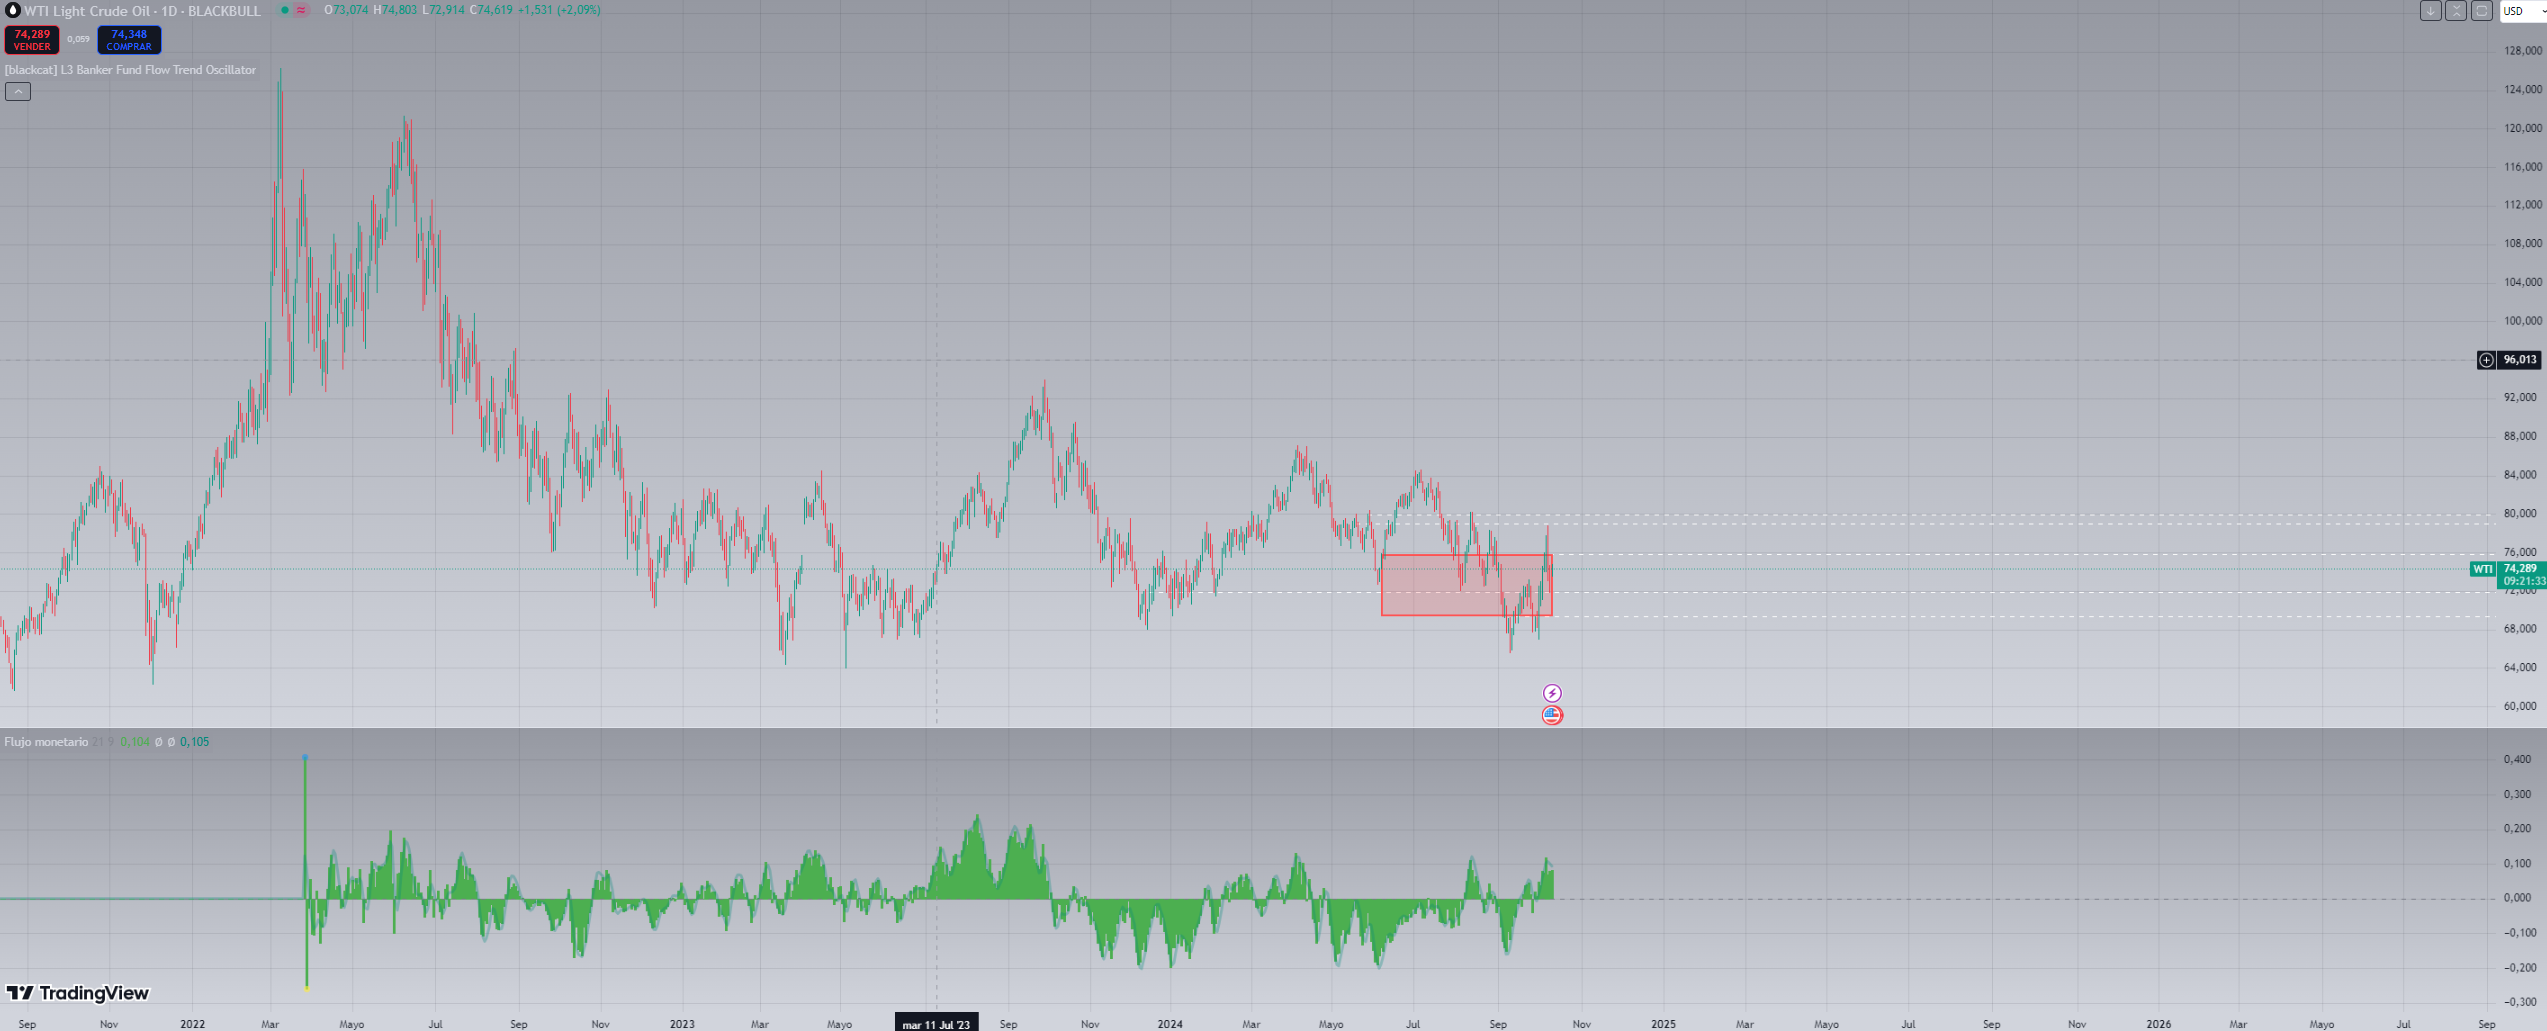
\includegraphics[width=0.8\textwidth]{images/Captura de pantalla 2024-10-10 133834.png}
\caption{Evolución reciente del precio del petróleo.}
\end{figure}

\begin{table}[h!]
\centering
\begin{tabular}{|c|c|c|}
\hline
Divisa & Correlación con el precio del crudo & Oportunidad de Trading \\
\hline
Ruble Ruso & 0.75 & Estrategia de cobertura \\
Dólar Canadiense & 0.60 & Oportunidad de arbitraje \\
\hline
\end{tabular}
\caption{Correlación entre divisas de exportadores de petróleo y el precio del crudo.}
\end{table}

\section{Riesgos Potenciales}
Existen varios riesgos clave que podrían afectar los mercados:
\begin{itemize}
    \item \textbf{Volatilidad Geopolítica:} Un aumento en las tensiones entre Irán e Israel podría generar disrupciones en el suministro de petróleo.
    \item \textbf{Políticas Económicas:} Cambios en las políticas de los gobiernos occidentales respecto a la liberación de reservas estratégicas de petróleo podrían provocar un aumento en los precios.
    \item \textbf{Eventos Inesperados:} Ataques a infraestructuras petroleras o cierres de rutas clave como el Estrecho de Ormuz podrían desatar movimientos alcistas bruscos.
\end{itemize}

\section{Estrategia Recomendada}
\subsection{Estrategia de Trading Basada en Correlación Sectorial}
Dada la baja prima de guerra en el precio del petróleo y el comportamiento lateral del mercado, una estrategia innovadora para maximizar el rendimiento en el corto plazo es la siguiente:
\begin{itemize}
    \item \textbf{Rotación Sectorial y Flujos de Capital:} Aprovechar la rotación sectorial entre energía y tecnología. Históricamente, cuando el sector energético se mantiene estancado, los inversores tienden a mover capitales hacia sectores como la tecnología. Se recomienda monitorear fondos sectoriales y seguir los flujos de capital entre estos sectores para posicionarse estratégicamente.
    \item \textbf{Estrategia de Arbitraje en Divisas:} Aprovechar la correlación entre divisas de países exportadores de petróleo y el precio del crudo. Esto incluye pares como el USD/RUB y USD/CAD. Operar en periodos de alta volatilidad en el crudo puede generar oportunidades de arbitraje entre estos pares.
\end{itemize}

\subsection{Estrategia de Indicadores No Convencionales}
Una técnica innovadora es utilizar indicadores de estrés financiero basados en la volatilidad y los eventos geopolíticos. Este enfoque implica monitorear la volatilidad implícita en los contratos de opciones sobre petróleo, buscando picos anormales que indiquen oportunidades de trading antes de que el mercado ajuste los precios.

\section{Conclusión}
El análisis de la situación actual del petróleo revela que, a pesar de la tensión geopolítica, el mercado ha respondido con calma debido a factores como el crecimiento de la producción en EE.UU. y la liberación de reservas. Sin embargo, esto presenta oportunidades estratégicas de arbitraje y rotación sectorial que pueden aprovecharse mediante análisis innovadores de flujos de capital y correlaciones de mercado.

\end{document}
